\subsection{Events}
To better understand the local system behavior, it is necessary to be aware of the events that may occur, defining how the system will respond to each one of them, as shown in table \ref{table:ls_events}. 
%The asynchronous events are generally triggered from external sources. In contrast, the synchronous events are triggered periodically.

\begin{table}[ht]
	\centering
	\resizebox{\columnwidth}{!}
	{
%	\begin{tabular}{||c | c | c | c||} 

	\begin{tabular}{|m{3cm}|m{5cm}|m{2.4cm}|m{2.4cm}|}
		\hline
		\textbf{Event} & \textbf{System Response} & \textbf{Source} & \textbf{Type}\\
		\hline\hline
		Low luminosity detected & Put lamp at a predefined minimum bright level & Environment & Asynchronous\\
		\hline
		
		Motion detected & Put lamp at maximum bright level & User & Asynchronous\\
		\hline
		
		LED failure detected & Notify remote system & Local system & Asynchronous\\
		\hline
		
		Requested to turn on the lamp & Put lamp at maximum bright level & Remote system & Asynchronous\\
		\hline
		
		Camera sample period & Acquire camera frame and do image processing & Timer & Synchronous\\
		\hline
		
		Sensors data acquisition & Sample sensor values & Timer & Synchronous\\
		\hline
		
		Update system information & Send data to remote system & Local system & Asynchronous\\
		\hline
	\end{tabular}
	}
	\caption{Events: Local System.}
	\label{table:ls_events}
\end{table}

\clearpage
\subsection{Use Cases}
The local system use cases are presented in figure \ref{fig:ls_use_cases}. A street passerby, a car or a pedestrian, can interact with each local system by moving in the vicinity of the lamppost, triggering it's motion detector, or by clearing a parking space.

\begin{figure}[ht] 
	\centering
	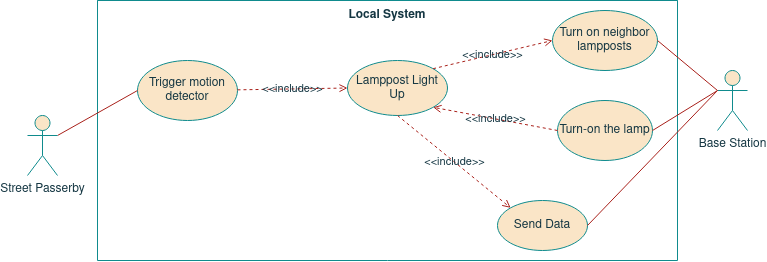
\includegraphics[width=1\textwidth]{/04local_system/LS_UseCase}
	\caption{Use Cases: Local System.}
	\label{fig:ls_use_cases}
\end{figure}

When movement is detected, the lamp is put at maximum bright level. The system then informs this occurrence to the remote system, through the gateway, in order to turn on the neighbor lampposts. The opposite can also happen, when a neighbor local system, with the lamp already on, requests this local system to turn on its lamp, being this request handled by the remote system. 

Moreover, the local system is periodically doing image processing after the capture of camera frames. So when the street passerby clears a parking space, the system will detect that, and will send that notification to the remote system.

\clearpage
\subsection{State Chart}
In figure \ref{fig:ls_state_chart} its represented the state chart of the local system. 

\begin{figure}[H]
	\centering
	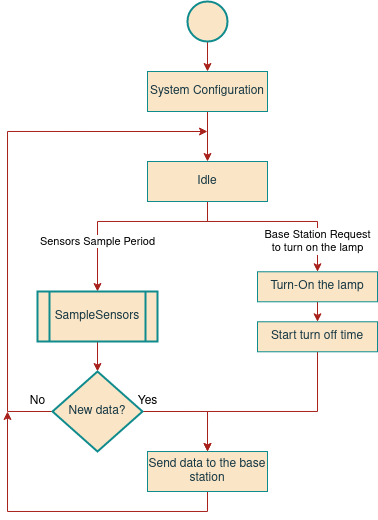
\includegraphics[width=1\textwidth]{/04local_system/LS_StateChart}
	\caption{State Chart: Local System.}
	\label{fig:ls_state_chart}
\end{figure}

It initiates with the system configuration, initializing all peripherals from this system, including the sensors, the camera, the LoRa communication module and the timer for sensors data acquisition. The timer is used to sample sensor values periodically and to acquire image frames through the camera. After that, the system enters an idle state.

When motion is detected and the luminosity sensor detects low luminosity conditions, for example, during the night, the lamp is put at its maximum bright level, for a predefined time window, and this information is sent to the remote server. When this time window passes, the lamp is put at a predefined minimum bright level, and again, informs the remote system of this event. Every time motion is detected, when the lamp is already on, the time window for the lamp being on is restarted.

To do the sensors data acquisition, including the camera frame sampling, are used sample periods, that periodically triggers the sampling of the sensors. In "SampleSensors" state, the system checks the luminosity sensor levels and if the LED failure detector hasn't detected a failure on the lamp. If a LED failure is detected, that information is sent to the remote system. To do the image processing, it is also used a sample period to get image frames through the camera. If there is an available parking space detected, that information is sent to the remote server.

When the local system detects that the remote system is sending a message, either to turn on the lamp of the local system, or other reason, the system goes to a dedicated state to receive that message.

\subsection{Sequence Diagram}
In figure \ref{fig:ls_seq_diagram} it is shown the local system sequence diagram. When a street passerby triggers the motion detector, the local system turns on its lamp, and, at that moment, using the communication management of the system, that information is sent to the remote system. If, no more movement is detected, the lamp turns off after a predefined time (turn off time), and again, the lamp status is updated in the remote system.

An alternative of an interaction with the local system is when the remote system requests the local system to turn on its lamp, this being processed in a similar way to the previous example, when the user triggers the motion detector. The remote system does this requests to local systems to dynamically turn on the lampposts as a passerby is walking down a street.

Note that, regarding the lamp control, one may use “turn on” to represent the lamp bright transition from minimum bright level to maximum bright level, and use “turn off” to represent the opposite, the transition from maximum bright level to minimum bright level. The lamp is only off when low luminosity conditions are not verified, i.e, during the day.

\begin{figure}[H]
	\centering
	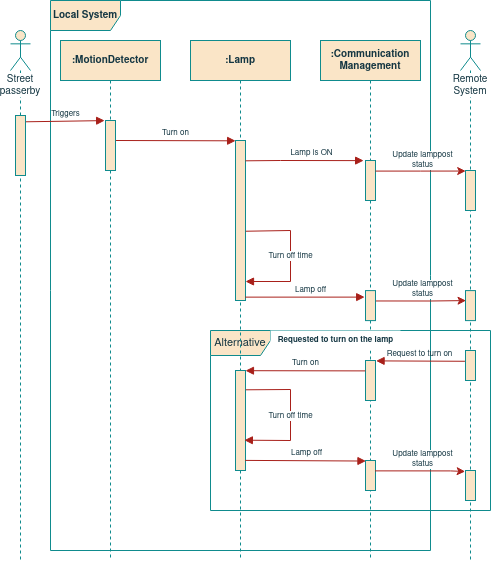
\includegraphics[width=0.9\textwidth]{/04local_system/LS_SeqDiagram}
	\caption{Sequence Diagram: Local System.}
	\label{fig:ls_seq_diagram}
\end{figure}

\clearpage
In figure \ref{fig:ls_seq_diagram_timer} it is shown the local system data acquisition sequence diagram. A timer is used to trigger two different samplings, one to sample sensor values, other to sample image frames from the camera. 

When the sensors sample period occurs, the sampling is started, gathering values from the luminosity sensor and from the LED failure detector. If a LED failure is detected, that is sent to the remote system through the communication management system.

When the camera sample period occurs, one gets an image frame from the camera and does image processing, in order to avail if there is an available parking spot. If that comes true, it's communicated to the remote system, like in the previous example.

\begin{figure}[H]
	\centering
	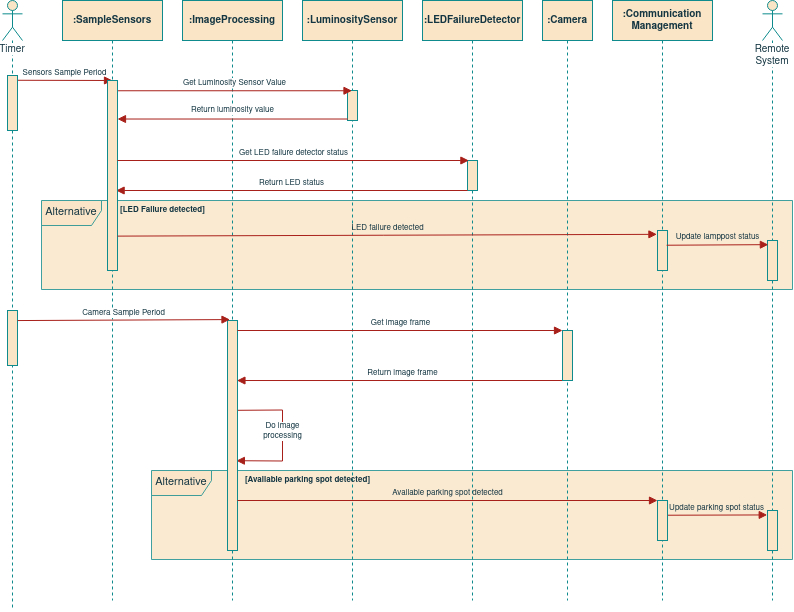
\includegraphics[width=1\textwidth]{/04local_system/LS_SeqDiagram_Timer}
	\caption{Sequence Diagram: Local System Data Acquisition.}
	\label{fig:ls_seq_diagram_timer}
\end{figure}